% Preprint draft (revision 4). Build instructions: README.md.
\documentclass[11pt]{article}
\usepackage[T1]{fontenc}
\usepackage[utf8]{inputenc}
\usepackage{lmodern}
\usepackage[a4paper,margin=1in]{geometry}
\usepackage{amsmath,amssymb,amsthm,mathtools}
\usepackage{microtype,booktabs,array,url,graphicx}
\usepackage[numbers,sort&compress]{natbib}
\usepackage{tikz}
\usetikzlibrary{arrows.meta,positioning}
\usepackage[colorlinks=true,linkcolor=blue!50!black,citecolor=green!40!black,urlcolor=blue!50!black]{hyperref}
\emergencystretch=3em
\newcolumntype{L}[1]{>{\raggedright\arraybackslash}p{#1}}
\theoremstyle{plain}
\newtheorem{theorem}{Theorem}
\newtheorem{proposition}[theorem]{Proposition}
\newtheorem{lemma}[theorem]{Lemma}
\newtheorem{corollary}[theorem]{Corollary}
\theoremstyle{definition}
\newtheorem{definition}{Definition}
\newtheorem{example}{Example}
\theoremstyle{remark}
\newtheorem{remark}{Remark}
\newcommand{\Stmt}{\mathcal E}
\newcommand{\Term}{\mathcal T}
\newcommand{\Iri}{\mathcal I}
\newcommand{\SG}{\mathsf{SG}}
\newcommand{\refs}{\prec}
\newcommand{\sys}[1]{\texttt{sys:#1}}
\newcommand{\iri}[1]{\texttt{#1}}
\newcommand{\Kernel}{\mathsf{K}}
\newcommand{\Close}{\mathsf{C}}
\newcommand{\Erase}{\mathsf{erase}}
\newcommand{\refset}{\mathsf{ref}}
\title{When Is a Temporal Statement Store a Statement Graph?\\[2pt]
\large Export Boundaries for Occurrence Records with Two Clocks}
\author{Volodymyr Pavlyshyn\\[2pt]\small Independent researcher\\
\small\href{mailto:pavlyshyn@tiramemsu.com}{pavlyshyn@tiramemsu.com}\quad
\small\href{https://tiramemsu.com}{tiramemsu.com}}
\date{Revision 4, 12 October 2026}
\hypersetup{pdftitle={When Is a Temporal Statement Store a Statement Graph?},pdfauthor={Volodymyr Pavlyshyn}}
\begin{document}
\maketitle

\begin{abstract}
A temporal statement store keeps every statement occurrence as a record with an
identifier, a triple, a transaction-time lifetime and a valid-time interval, and
lets other records refer to it. We ask which part of such a store can be exported
as a Statement Graph, the DAG model that underlies OneGraph interoperability
between RDF-star and property graphs, without inventing or renaming any occurrence.
The answer has three parts. \emph{What can be exported:} a selected record set
admits an identity-preserving export exactly when it is closed under references and
acyclic, and every set contains a greatest such subset, the least fixpoint of a
one-line operator, computed by a linear-time topological peel that also yields an
export order. When content is immutable, records are never deleted and inserts
reference only existing records, the whole history is closed, so exporting the history rather than a snapshot loses only cycles created by
atomic correction, and a per-record bit maintained at insert time turns export into
a filter scan; a batch-local check at correction time removes even those cycles.
\emph{What is dropped:} snapshot export additionally drops
supersession lineage, whose targets are retracted; a dual reference-closure keeps it
by adding the retracted targets. \emph{What is reported:} every omitted record with
a reason. An explicit encoding into the RDF-star branch of the OneGraph image, with
transaction and valid time as reserved statements, makes the roundtrip of the
exportable history lossless, and conjunctive queries over the asserted part are answered
identically up to a quoting bijection. Two contrasts locate the boundary: RDF~1.2
reifiers name occurrences instead of nesting them and need neither closure nor
acyclicity, but assert per triple, not per occurrence; the property-graph branch
admits only edges and unreferenced properties, so it carries both clocks for edges
alone. Proofs are by hand; a validator checks the constructions on exhaustive small
stores and random protocol histories, and both counterexamples are traced through
the tiramemsu engine.
\end{abstract}

\section{Introduction}
RDF identifies resources globally and represents a graph as a set of triples.
Labeled property graphs (LPGs) give nodes and edges identity and attach properties
to them. Statement-level information complicates translation between the two:
occurrence identity, annotations and the meaning of updates need not survive a
surface view. The OneGraph vision names these problems, including the ambiguity of
deleting one visible triple backed by several occurrences \cite{lassila2023onegraph}.
Statement Graphs make the shared structure explicit as a directed acyclic graph
whose internal vertices are statements with subject, predicate and object edges
\cite{gelling2023bridging,gelling2024statement}.

A temporal store can hold a statement vertex and its three role edges in one
record. The embedded database tiramemsu \cite{tiramemsu2026} uses
\[
(e,s,p,o,a,d,v_1,v_2),
\]
where $e$ identifies an occurrence, $(s,p,o)$ is its content, $[a,d)$ is its
transaction-time lifetime and $[v_1,v_2)$ its valid-time interval. Subjects and
objects may be identifiers of other records. The record shape suggests that the
store \emph{is} a Statement Graph. It is not, in general, and this paper says
exactly when it is and what to do when it is not.

\paragraph{Running example.}
At transaction~1 we assert a route and annotate it with its distance:
\[
e_1=(\iri{:FRA},\iri{:route},\iri{:LHR}),\qquad e_2=(e_1,\iri{:distance},655).
\]
These two records translate to two statement vertices; the second points at the
first. At transaction~2 the route's valid time is corrected. The engine retracts
$e_1$ and its dependent $e_2$, replays them under fresh identifiers $e_1',e_2'$,
and records lineage $\ell=(e_1',\sys{supersedes},e_1)$. The current snapshot
$\{e_1',e_2',\ell\}$ is not a Statement Graph: $\ell$ points at the retracted $e_1$.
The full history $\{e_1,e_2,e_1',e_2',\ell\}$ is. A different correction, whose
patched object names the annotation $e_2$, replays into
$e_1'=(\iri{:FRA},\iri{:route},e_2')$ and $e_2'=(e_1',\iri{:distance},655)$, a
two-cycle that neither the snapshot nor the history can export directly
(Examples~\ref{ex:lineage} and~\ref{ex:cycle}).

\paragraph{Contributions.}
\begin{enumerate}
\item A formal notion of identity-preserving direct export and a theorem: it exists
exactly for closed, acyclic record sets (Theorem~\ref{thm:criterion}).
\item The \emph{export kernel}, the least fixpoint of
$F_S(X)=\{r\in S:\refset(r)\subseteq X\}$, which is the unique greatest closed,
acyclic subset; a linear-time peel computing it with an export order; and
incremental maintenance by one bit per record (Section~\ref{sec:kernel}).
\item The dual \emph{reference closure}, the least closed superset within the
history, which keeps lineage that the kernel drops (Section~\ref{sec:dual}).
\item Full-history results: under append-only content and no deletion the history is
closed and its cycles lie inside single replay batches, so the history kernel drops
only replay cycles and their dependents (Section~\ref{sec:history}).
\item An explicit encoding into the RDF-star branch of the OneGraph image, extended
with reserved time statements to a lossless roundtrip of the exportable bitemporal
history (Section~\ref{sec:encoding}), and a query-preservation result for
conjunctive queries over its asserted part (Section~\ref{sec:queries}).
\item Two boundary contrasts: an RDF~1.2 reifier encoding that exports every store,
cycles included, and the exact direct-export condition for the property-graph
branch (Section~\ref{sec:other}).
\item An acyclic-replay rule, checkable on the replay batch alone, under which the
whole history is always exportable (Section~\ref{sec:history}).
\item A validator over exhaustive and random stores and protocol histories, and
engine traces of both running-example corrections (Section~\ref{sec:validation}).
\end{enumerate}
The graph facts used are elementary: the kernel is the well-founded part of the
reference relation, and its computation is Kahn's topological sort
\cite{kahn1962topological}. The contribution is their application to temporal
statement stores, and their value is in the engine invariants they license: which
subset to export, which rule a writer must enforce so that nothing is lost, what one
stored bit buys, what an exporter must report, and how time travels with it.

\paragraph{Relation to earlier work.}
The first companion paper develops temporal integrity, the distinction between
structural and lineage references, and correction contracts
\cite{pavlyshyn2026lbg}; the second studies exact images of metagraph encodings
\cite{pavlyshyn2026metagraphenc}. A site article explains the row/vertex
correspondence informally \cite{pavlyshyn2026statementarticle}. This paper reuses
their occurrence model. Its new material is the export kernel and its fixpoint
characterization, the reference closure, the full-history results and the temporal
encoding.

\section{Statement Graphs and their RDF-star image}\label{sec:background}
We use the definitions of Gelling, Fletcher and Schmidt in the arXiv version
\cite{gelling2023bridging}; the DASFAA paper \cite{gelling2024statement} is its
published form.

\begin{definition}[Statement Graph {\cite[Def.~4.1]{gelling2023bridging}}]
A Statement Graph is a finite directed acyclic graph with injectively labeled
vertices. An internal vertex is labeled by a statement identifier and has exactly
one outgoing edge of each role: subject, predicate, object. A leaf is labeled by a
concrete value, has no outgoing edges and at least one incoming edge.
\end{definition}

The RDF-star image \cite[Def.~5.1]{gelling2023bridging} adds typing and membership
conditions. Subject targets are statements, IRIs or blank nodes; predicate targets
are IRIs; object targets are statements, IRIs, blank nodes or literals. A reserved
IRI $\mathit{in}$ marks \emph{membership statements} $(v,\mathit{in},g)$, which
assign a triple statement $v$ to a graph name or the default graph identifier $g$.
A membership statement has a statement subject, an IRI or blank-node object and no
incoming edges. Every other statement vertex has at least one incoming edge, and no
two vertices are isomorphic. The membership condition is what distinguishes an
asserted triple, which some membership places in a graph, from a triple that only
occurs as a quoted term. The OneGraph image \cite[Def.~5.4]{gelling2023bridging}
requires each connected component to be an RDF-star image or an LPG image,
disregarding the isomorphism condition. We target its RDF-star branch.

The Neptune Analytics demo uses OneGraph concepts, relationship and property
statements and openCypher updates over RDF \cite{schmidt2024opencypher}; nothing
below depends on its internal model.

\section{Records and identity-preserving export}\label{sec:model}
Let $\Term$ be the disjoint union of IRIs $\Iri$, local node identifiers, blank
nodes, literals $\mathcal L$ and transaction identities, and let $\Stmt$ be a
disjoint set of occurrence identifiers (eids). Valid time ranges over
$\mathbb Z\cup\{-\infty,+\infty\}$; transaction numbers are positive integers.

\begin{definition}[Record, store, snapshot, references]
A record is $r=(e,s,p,o,a,d,v_1,v_2)$ with $e\in\Stmt$,
$s\in(\Term\setminus\mathcal L)\cup\Stmt$, $p\in\Iri$, $o\in\Term\cup\Stmt$,
$a\ge1$, $d=\bot$ or $d\ge a$, and $v_1<v_2$. A store $D$ is a finite set of
records with distinct eids. Its committed snapshot at $t$ is
$D@t=\{r\in D:a_r\le t\text{ and }(d_r=\bot\text{ or }t<d_r)\}$.
The references $\refset(r)\subseteq\Stmt$ are the eid endpoints of $r$, and
$r\refs r'$ when $e_{r'}\in\refset(r)$. A set $S\subseteq D$ is \emph{closed} if
$\refset(r)\subseteq e(S)$ for every $r\in S$, and \emph{acyclic} if $\refs$
restricted to $S$ has no directed cycle.
\end{definition}

Write $\Erase(S)=\{(e,s,p,o):r\in S\}$ for temporal erasure; unlike projection to
$(s,p,o)$, it keeps occurrence identity. Fix an injective map $f$ from source
terms to target terms that preserves literals and blank nodes and sends every other
term to an IRI.

\begin{definition}[Identity-preserving direct export]\label{def:direct}
An identity-preserving direct export of $S$ is a Statement Graph $G$ such that
(a) the internal vertices of $G$ are exactly one vertex labeled $e_r$ for each
$r\in S$; and (b) for each $r\in S$ and role $\rho\in\{s,p,o\}$, if $r.\rho$ is an
eid $x$, the $\rho$-edge of $e_r$ targets the internal vertex labeled $x$, and
otherwise it targets a leaf labeled $f(r.\rho)$.
\end{definition}

Condition (a) forbids inventing occurrences, including referents absent from $S$.
Condition (b) forbids rewriting a reference into anything other than the
referenced occurrence.

\begin{theorem}[Exact direct-export criterion]\label{thm:criterion}
$S$ has an identity-preserving direct export if and only if $S$ is closed and
acyclic. The export is then unique; call it $\SG(S)$. Reading the three role
targets of each internal vertex and applying $f^{-1}$ to leaves recovers
$\Erase(S)$.
\end{theorem}
\begin{proof}
($\Leftarrow$) Build one internal vertex per record and one leaf per distinct term
$f(t)$ occurring in $S$, and add the role edges required by (b). Closure supplies
every internal target. Distinct eids, injectivity of $f$ and disjointness of $\Stmt$
and $\Term$ give injective labels; each leaf has an incoming edge by construction.
Edges between internal vertices are exactly references, and leaves have no
outgoing edges, so the graph is acyclic because $S$ is.

($\Rightarrow$) Let $G$ satisfy (a) and (b). If $x\in\refset(r)$ for some $r\in S$,
(b) requires an internal vertex labeled $x$, and by (a) that is $e_{r'}$ for some
$r'\in S$; hence $S$ is closed. By (b) every reference $r\refs r'$ is an edge
between internal vertices, so a reference cycle in $S$ is a cycle in $G$, which a
Statement Graph does not have.

Uniqueness: (a) and (b) fix all internal vertices and all edges; a leaf has an
incoming edge, so the leaves are exactly the targets named in (b). Recovery reads
each vertex's three targets independently.
\end{proof}

\begin{remark}[Leaf substitution]
For a nonclosed $S$ one can still obtain a Statement Graph by reading a dangling eid
$x$ as a leaf, for instance an IRI naming $x$. That graph violates (b), and a
consumer cannot tell a reference to an absent occurrence from an ordinary term. The
validator checks this on an explicit case.
\end{remark}

\section{The export kernel}\label{sec:kernel}
Fix a selected set $S$, typically a snapshot $D@t$ or the history $D$. We admit
only the deletion of whole records: no endpoint substitution, no new referents and
no change of identifiers. For $X\subseteq S$ define
\[
F_S(X)=\{r\in S:\refset(r)\subseteq e(X)\},
\qquad
\Kernel(S)=\bigcup_{k\ge0}F_S^{\,k}(\emptyset).
\]
$F_S$ is monotone, so the chain $F_S^k(\emptyset)$ increases and stabilizes after at
most $|S|$ steps at the least fixpoint of $F_S$. The \emph{rank} of $r\in\Kernel(S)$
is the least $k$ with $r\in F_S^k(\emptyset)$. Records without references have
rank~1.

\begin{theorem}[Greatest direct-export subset]\label{thm:kernel}
$\Kernel(S)$ is the unique greatest closed, acyclic subset of $S$. Consequently
$\SG(\Kernel(S))$ exists, $\Kernel(S)=S$ exactly when $S$ is closed and acyclic,
$\Kernel$ is idempotent, and $S\subseteq S'$ implies $\Kernel(S)\subseteq\Kernel(S')$.
\end{theorem}
\begin{proof}
\emph{Closed:} $\Kernel(S)=F_S(\Kernel(S))$, so every reference of a kernel record
lands in the kernel. \emph{Acyclic:} a record of rank $k$ lies in
$F_S(F_S^{k-1}(\emptyset))$, so its references have rank below $k$; references
strictly decrease rank, which no cycle can do. \emph{Greatest:} let $U\subseteq S$
be closed and acyclic. For $r\in U$ let $h(r)$ be the length of the longest
reference path from $r$ inside $U$; it is finite because $U$ is finite and
acyclic, and closure keeps every reference of $r$ inside $U$ with smaller $h$. By
induction on $h$, $r\in F_S^{h(r)+1}(\emptyset)$: if $h(r)=0$ then
$\refset(r)=\emptyset$, and otherwise all references of $r$ are in
$F_S^{h(r)}(\emptyset)$. Hence $U\subseteq\Kernel(S)$. Uniqueness of a greatest
element is immediate, and the remaining claims follow: $S$ itself qualifies exactly
when it is closed and acyclic; the kernel is closed and acyclic, so it is its own
kernel; and $F_S\subseteq F_{S'}$ pointwise when $S\subseteq S'$.
\end{proof}

The kernel is the well-founded part of $\refs$ on $S$, where a missing target
counts as non-well-founded. It is the dual of reachability garbage collection
\cite{jones1996gc}: a collector keeps what roots reach, the kernel keeps what reaches
only grounded records. The obstruction form explains omissions.

\begin{corollary}[Obstructions]\label{cor:obstructions}
Let $B\subseteq S$ consist of the records with a reference outside $e(S)$ and the
records on a directed reference cycle in $S$, and let $A$ be the records of $S$ that
reach $B$ (zero-length paths included). Then $\Kernel(S)=S\setminus A$.
\end{corollary}
\begin{proof}
$S\setminus A$ is closed, since a retained record has no missing target and does
not reach $A$; and acyclic, since cycle vertices are in $B$. Hence
$S\setminus A\subseteq\Kernel(S)$. Conversely a closed, acyclic set contains no
record with a missing target, no cycle vertex (closure would pull in the whole
cycle) and, by repeated closure, no record reaching either.
\end{proof}

\paragraph{Algorithm.}
For each record count its references; a record with a reference outside $e(S)$ is
never ready. Queue the records whose count is zero. Repeatedly pop a record, append
it to the output order, and decrement the count of each record that references it,
queuing those that reach zero. The popped records are $\Kernel(S)$ and the output
order lists every record after all its targets, which is the order a streaming
RDF-star or Statement Graph writer needs. With indexed eid lookup this takes
$O(n+m)$ time, where $n=|S|$ and $m\le2n$ counts reference positions. Records never
popped form $A$. Reporting a reason for each omission (missing target $x$, on a
cycle, or depends on omitted $y$) needs one strongly connected component pass over
$A$ only. Revision~2 of this paper computed $\Kernel$ from components first; the
validator keeps that version as an independent implementation.

\begin{figure}[t]
\centering
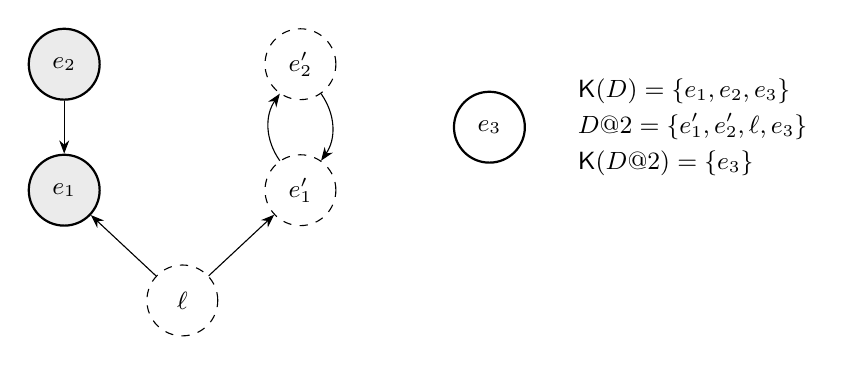
\begin{tikzpicture}[>=Stealth,
 kept/.style={circle,draw,thick,minimum size=9mm},
 hist/.style={circle,draw,thick,fill=black!8,minimum size=9mm},
 removed/.style={circle,draw,dashed,minimum size=9mm},
 font=\small]
\node[hist] (e1) at (0,0) {$e_1$};
\node[hist] (e2) at (0,1.6) {$e_2$};
\draw[->] (e2) -- (e1);
\node[removed] (f1) at (3,0) {$e_1'$};
\node[removed] (f2) at (3,1.6) {$e_2'$};
\draw[->] (f1) to[bend left=35] (f2);
\draw[->] (f2) to[bend left=35] (f1);
\node[removed] (l) at (1.5,-1.4) {$\ell$};
\draw[->] (l) -- (f1);
\draw[->] (l) -- (e1);
\node[kept] (e3) at (5.4,0.8) {$e_3$};
\node[align=left,anchor=west] at (6.4,0.8) {$\Kernel(D)=\{e_1,e_2,e_3\}$\\[2pt]
$D@2=\{e_1',e_2',\ell,e_3\}$\\[2pt]$\Kernel(D@2)=\{e_3\}$};
\end{tikzpicture}
\caption{History of the cyclic correction (Example~\ref{ex:cycle}) with an
unrelated fact $e_3$. Arrows go from referring records to their targets; term
endpoints are suppressed. Shaded records are retracted at transaction~2; dashed
records are outside $\Kernel(D)$. The history kernel keeps the pre-correction
records; the snapshot kernel keeps only $e_3$, because $\ell$ also dangles there.}
\label{fig:kernel}
\end{figure}

\paragraph{What the kernel does and does not do.}
Closure makes removing one edge of a cycle inadmissible: both records of a
two-cycle and all their dependents go, while unrelated facts stay
(Figure~\ref{fig:kernel}). The kernel does not maximize business value or
reproduce query answers over the omitted records. An exporter should return the
omitted eids with reasons, and a caller that needs completeness should reject an
incomplete export rather than use the kernel silently. Dropping lineage predicates
by name is not a substitute: retained records may still reference dropped lineage
occurrences.

\section{The reference closure}\label{sec:dual}
The kernel deletes. The opposite design keeps every selected record and adds the
historical records it references.

\begin{definition}[Reference closure]
For $S\subseteq D$, $\Close_D(S)$ is the set of records of $D$ reachable from $S$
along $\refs$, including $S$; it is defined when every reachable eid belongs to a
record of $D$.
\end{definition}

\begin{proposition}[Least closed superset]\label{prop:dual}
If $D$ is closed, $\Close_D(S)$ is defined and is the least closed subset of $D$
containing $S$. Moreover
$\Kernel(S)\subseteq\Kernel(\Close_D(S))\subseteq\Close_D(S)$, and every record of
$S$ in $\Kernel(\Close_D(S))\setminus\Kernel(S)$ was omitted from $\Kernel(S)$ only
because some record it reaches lies outside $S$.
\end{proposition}
\begin{proof}
Reachability from $S$ is closed by construction, and any closed superset of $S$
contains everything $S$ reaches. The inclusions are monotonicity of $\Kernel$
(Theorem~\ref{thm:kernel}). For the last claim, let $r\in S\cap\Kernel(\Close_D(S))$. By
Corollary~\ref{cor:obstructions}, no record that $r$ reaches in $\Close_D(S)$ has a
missing target or lies on a cycle. If every record $r$ reaches were in $S$, then $r$
would reach the same records in $S$, none of them an obstruction in $S$, and $r$
would be in $\Kernel(S)$.
\end{proof}

For $S=D@t$ the added records $\Close_D(S)\setminus S$ are retracted at or before
$t$, and an exporter should mark them so (Section~\ref{sec:encoding} encodes this
as the absence of a membership). In Example~\ref{ex:lineage},
$\Kernel(D@2)=\{e_1',e_2'\}$ silently drops the supersession provenance $\ell$,
whereas $\Close_D(D@2)=\{e_1,e_1',e_2',\ell\}$ is exportable as a whole and keeps
it, with $e_1$ marked retracted. The reference closure therefore costs extra
historical records and requires consumers to respect the retraction marks; the
kernel costs provenance. A store with acyclic history can offer the closure with no
omissions at all.

\section{Temporal operations and the full history}\label{sec:history}
A storage protocol and an export validator do different jobs: the protocol may
admit structures the exporter must reject. This section states which structures a
temporal store can produce. Four commitments of tiramemsu matter; the remaining
design commitments are listed in Appendix~\ref{app:commitments}.

\begin{description}
\item[C3 Live references.] An ordinary insert at $t$ may reference only records live
at that moment. Engine-written lineage may reference allocated historical records.
\item[C4 Immutable history.] Content and identifiers never change, records are never
deleted and $d$ is set at most once; the file enforces this with triggers.
\item[C5 Cascade.] Retracting a record retracts its live transitive dependents in
the same transaction.
\item[C6 Correction by replay.] Supersession retracts the cascade set $C$ of a root,
preallocates fresh eids $\sigma$ for the retained members, inserts each retained
member with its references into $C$ rewritten through $\sigma$ (the root also receives the patch, itself
rewritten through $\sigma$), and inserts lineage $(\sigma(\mathit{root}),\sys{supersedes},\mathit{root})$.
\end{description}

\subsection{Snapshots}
Call the \emph{restricted protocol} transactions numbered in increasing order whose
operations are inserts obeying C3 and retractions obeying C5, with C4 throughout and
no supersession.

\begin{proposition}[Snapshot closure]\label{prop:closure}
Under the restricted protocol every committed snapshot is closed and the history
is acyclic.
\end{proposition}
\begin{proof}
Induct on operations within a transaction. An insert references live records. If a
retraction removed the target of a remaining live record, that record would be a
dependent and would have been retracted too. With $I_t$ the records inserted and
$R_t$ those retracted during $t$, the committed snapshot is
$(D@(t-1)\cup I_t)\setminus R_t$; records inserted and retracted within $t$ have
$a=d=t$ and an empty lifetime. Acyclicity: rank records by insertion; every
reference points to an earlier insertion.
\end{proof}

Valid-time selection may still break closure: a present dispute about an expired
contract can have a valid interval outside the contract's.

\begin{example}[Historical lineage]\label{ex:lineage}
Correct the valid time of $e_1$ in the running example. Supersession retracts
$\{e_1,e_2\}$, inserts $e_1'$ with the new valid time, $e_2'=(e_1',\iri{:distance},655)$
and $\ell=(e_1',\sys{supersedes},e_1)$. Then $D@2=\{e_1',e_2',\ell\}$ is not closed
and $\Kernel(D@2)=\{e_1',e_2'\}$, while the history $D$ is closed and acyclic, so
$\Kernel(D)=D$.
\end{example}

\begin{example}[Correction-generated cycle]\label{ex:cycle}
Instead supersede $e_1$ with an object patch naming $e_2$. The patch is rewritten
through $\sigma$, giving $e_1'=(\iri{:FRA},\iri{:route},e_2')$ and
$e_2'=(e_1',\iri{:distance},655)$, plus $\ell$. Neither record refers to itself;
together they form a two-cycle. The engine rejects a direct self-reference but
accepts this case, and its regression test pins that behavior. Here
$\Kernel(D)=\{e_1,e_2\}$ and $\Kernel(D@2)=\emptyset$.
\end{example}

\subsection{The full history}
Exporting $D$ rather than $D@t$ removes the dangling-lineage failure entirely.

\begin{proposition}[Closed history]\label{prop:history}
Under C3--C6 the history $D$ is closed after every committed transaction, and every
directed reference cycle of $D$ consists of records inserted by one replay.
Consequently $\Kernel(D)$ is $D$ minus the replay cycles and the records that reach
them, and $D$ is acyclic whenever no replay creates a cycle.
\end{proposition}
\begin{proof}
Every reference written by an insert targets a live record (C3), a fresh eid of the
same replay that is inserted in the same transaction (C6), or, for lineage, an
allocated historical record. By C4 no record leaves $D$, so all these targets remain
in $D$. For cycles, order the inserts of a history by position, giving all records
of one replay the same position. An ordinary insert or a lineage record references
strictly earlier positions; a replayed record references earlier positions or its
own batch. Hence a cycle cannot leave one batch. The description of $\Kernel(D)$ is
Corollary~\ref{cor:obstructions} with no missing targets.
\end{proof}

Two practical consequences follow. First, cycles can be prevented where they arise.

\begin{definition}[Acyclic-replay rule]\label{def:strict}
Before a supersession writes anything, build the replay batch
$B=\{\sigma(c):c\in C\}$ with its rewritten references, treat references outside
$B$ as resolved, and peel $B$. If the peel leaves a record, abort the transaction.
\end{definition}

\begin{proposition}[Acyclic history]\label{prop:strict}
Under C3--C5, and C6 restricted by the acyclic-replay rule, $D$ is closed and acyclic
after every committed transaction, so $\Kernel(D)=D$, every exportable bit of
Proposition~\ref{prop:bit} is set, and the full history exports with no omissions.
The check costs $O(|C|)$ beyond the replay itself.
\end{proposition}
\begin{proof}
Closure is Proposition~\ref{prop:history}. A cycle of $D$ lies inside one replay
batch; references leaving the batch cannot be on it. The peel of
Section~\ref{sec:kernel} over $B$ with external references resolved leaves a
record exactly when $B$ contains a cycle or reaches one inside $B$, so an accepted
batch contains no cycle. The batch has $|C|$ records with at most two references
each.
\end{proof}

Under the rule the earlier history is acyclic, so the rewritten references among
$B$ copy an acyclic structure, and only the patch can add a cycle. Since every
member of $C$ reaches the root, a patch naming a member $c$ always closes the cycle
$\sigma(\mathit{root})\refs\sigma(c)\refs^{*}\sigma(\mathit{root})$ (a self-reference
when $c$ is the root). The rule therefore rejects exactly the patches that name a
member of $C$, as in Example~\ref{ex:cycle}, and the abort happens before any
retraction, with the offending member as its reason. tiramemsu~0.4.0 does not apply the rule: replay
substitutes the patch through $\sigma$ uniformly, and the resulting cycle is live
and closed, so the engine's own invariants (live endpoints, cascade, immutability)
hold for it and do not call for rejection. Its regression test pins this
behavior, and the engine rejects only a direct self-reference. Export is the first
consumer that needs a DAG. The theorems cover both policies: with the rule,
Proposition~\ref{prop:strict} applies; without it, Proposition~\ref{prop:history}
bounds the loss to replay cycles and their dependents. The validator runs the
protocol under both (Section~\ref{sec:validation}). We know of no use case that
needs a correction cycle, and we recommend the rule for stores that export.

Second, the kernel can be maintained incrementally.

\begin{proposition}[Exportable bit]\label{prop:bit}
Assign each record a bit when its transaction commits: peel the records inserted by
that transaction, treating references to earlier records as resolved exactly when
their bits are set. Under C3--C6 the set bit marks exactly $\Kernel(D)$ at every
commit, and no bit ever changes. If a snapshot $D@t$ is closed, $\Kernel(D@t)$ is
$D@t$ filtered by the bit.
\end{proposition}
\begin{proof}
A record references only records of its own or earlier transactions, so
$F_D$ restricted to earlier records is $F$ of the earlier history, and by induction their
kernel membership is unchanged by later inserts. Within the new batch the peel
computes the least fixpoint with the earlier bits fixed. For a closed snapshot,
everything a record of $D@t$ reaches lies in $D@t$, so by
Corollary~\ref{cor:obstructions} its kernel membership is the same in $D@t$ and
in $D$.
\end{proof}

Full-history export is thus a filter scan on one stored bit, and snapshot export is
the same scan plus live filtering, except where lineage dangles. Table~\ref{tab:ops}
states the per-operation invariants.

\begin{table}[t]
\centering\small
\caption{Per-operation invariants in tiramemsu~0.4.0. ``Model'' is checked by the
protocol simulation of \texttt{validate.py}; ``Engine'' names engine tests.}
\label{tab:ops}
\begin{tabular}{@{}L{2.0cm}L{6.4cm}L{5.8cm}@{}}
\toprule
Operation & Invariant & Checked by \\
\midrule
Assert, create & New references $\subseteq e(D@t)$; preserves closure of $D@t$ and $D$; adds no cycle & Model; Engine: statement endpoints must be live \\
Confirm, membership & Bearer and eid graph name live; same invariant as assert & Engine documentation \\
Bundle import & Topological order; cyclic bundles rejected; adds no cycle & Engine: import rejects cycles \\
Retract & Removes all live transitive dependents; preserves closure of $D@t$; $D$ unchanged except $d$ & Model \\
Supersede & References $\subseteq\sigma(C)\cup e(D@t)\cup\{\mathit{root}\}$; preserves closure of $D$; may break closure of $D@t$; cycles only inside $\sigma(C)$ & Model; Engine: correction remaps patched references; export boundary traces \\
\bottomrule
\end{tabular}
\end{table}

\section{OneGraph encodings}\label{sec:encoding}
We fix an encoding for any closed, acyclic $S$, in particular $\Kernel(D@t)$,
$\Kernel(\Close_D(D@t))$ and $\Kernel(D)$, and then extend it with time.

\paragraph{Dictionary.}
In tiramemsu a natural choice of $f$ keeps IRIs, literals and blank nodes and maps
engine-local identifiers to IRIs scoped by the database, for instance
\iri{urn:tiramemsu:<db-uuid>:n/<id>} for nodes and
\iri{urn:tiramemsu:<db-uuid>:tx/<t>} for transaction terms. The reserved IRIs below
must not occur in the image of $f$; source IRIs that clash are renamed and the
renaming is recorded in the dictionary. The dictionary is part of the decoding
contract.

\begin{definition}[Structural encoding $E_f$ and decoder $R_f$]\label{def:encoding}
Emit $\SG(S)$ with term leaves $f(t)$. For each record $e$ add one fresh membership
statement $m_e=(e,\mathit{in},G_D)$ for a reserved default-graph IRI $G_D$, without
adding memberships to memberships. Then $R_f$ removes the statements with predicate
$\mathit{in}$ and reads the remaining role targets, applying $f^{-1}$ to leaves.
\end{definition}

The memberships are required by the RDF-star image: a non-membership statement needs
an incoming edge, and a record that nothing references has none. They also say that
each exported record is asserted, rather than merely quoted. The cost is one extra
statement vertex per record.

\begin{theorem}[Image membership and structural roundtrip]\label{thm:image}
$E_f(S)$ belongs to the OneGraph image, and to the RDF-star image exactly when no two
records of $S$ share $(s,p,o)$. Moreover $R_f(E_f(S))=\Erase(S)$.
\end{theorem}
\begin{proof}
Typing: subjects are nonliteral terms or statements, predicates are IRIs other than
$\mathit{in}$, objects are any allowed term or statement. Every record vertex has an
incoming membership edge; every membership has a statement subject, an IRI object
and no incoming edge, since freshness prevents any record from referencing it.
$\SG(S)$ is acyclic and memberships are new roots, so $E_f(S)$ is acyclic; labels are
injective and every leaf is used. These are the RDF-star conditions other than
non-isomorphism, so each component meets the OneGraph condition. Two record vertices
are isomorphic exactly when their content agrees, by injectivity of $f$; memberships
have distinct subjects and a reserved predicate, so they are never isomorphic to
each other or to a record vertex. Decoding removes exactly the memberships and
inverts $f$.
\end{proof}

\paragraph{Temporal encoding.}
Reserve four further IRIs $\tau_a,\tau_d,\tau_1,\tau_2$. For a closed, acyclic $S$
and a set $\mathcal A\subseteq S$ of records to present as asserted, $T_f(S,\mathcal A)$
consists of $\SG(S)$ with leaves $f(t)$; for each record $e$ the time statements
$(e,\tau_a,a)$, $(e,\tau_d,d)$ if $d\ne\bot$, $(e,\tau_1,v_1)$ if
$v_1\ne-\infty$ and $(e,\tau_2,v_2)$ if $v_2\ne+\infty$, with integer literal
objects and fresh identifiers; a membership for every time statement; and a
membership $m_e$ exactly for $e\in\mathcal A$. The decoder $R^\tau_f$ removes
memberships, recording which records carried one, groups time statements by
subject, and restores each record with $\bot$ or $\pm\infty$ for absent clocks.

\begin{theorem}[Lossless temporal roundtrip]\label{thm:temporal}
$T_f(S,\mathcal A)$ belongs to the OneGraph image, and to the RDF-star image exactly
when no two records of $S$ share $(s,p,o)$. Moreover
$R^\tau_f(T_f(S,\mathcal A))=(S,\mathcal A)$, with all eight fields of every record.
\end{theorem}
\begin{proof}
The time statements have a record subject, a reserved IRI predicate and a literal
object, are referenced by nothing but their own memberships, and so add neither
cycles nor dangling edges. Every record vertex has an incoming edge from its
$\tau_a$ statement whether or not it carries a membership, so the incoming-edge
condition holds for records outside $\mathcal A$; this is exactly the RDF-star
reading of a quoted, unasserted triple. Time statements differ from one another
and from record vertices by subject or reserved predicate, so isomorphism can only
arise between records with equal content. The argument of Theorem~\ref{thm:image}
gives the rest; decoding inverts each step, and $\mathcal A$ is recovered from the
record memberships.
\end{proof}

With $S=\Kernel(D)$ this is a lossless roundtrip of the exportable bitemporal
history, and of the whole history when $D$ is acyclic
(Proposition~\ref{prop:history}). Two choices of $\mathcal A$ are natural.
Taking $\mathcal A=S$ presents every occurrence, including retracted ones, as
asserted; RDF-star consumers that ignore $\tau_d$ then see retracted facts as true.
Taking $\mathcal A=S\cap D@t$ asserts the snapshot and quotes history; consumers
that ignore time see exactly the snapshot, and the history remains attached as
statements about quoted triples. This matches the RDF~1.2 separation of a
proposition from its assertion \cite{w3c2026rdf12concepts}; Section~\ref{sec:other}
compares the two encodings. Each record costs up to nine
additional statement vertices; sharing one time statement per distinct clock value
would reduce that, at the price of a less direct decoder.

\paragraph{Graph memberships of the source.}
A tiramemsu membership $(m,e,\sys{inGraph},g)$ is an ordinary record and is encoded
as an ordinary triple, so its annotations and statement-valued graph names survive
structurally. Its native named-graph meaning is not mapped to the target
$\mathit{in}$; recovering the source dataset view is a separate interpretation step
after decoding.

\section{What queries see}\label{sec:queries}
A structural roundtrip says nothing about answers. We state what a time-unaware
RDF-star consumer of $T_f(S,\mathcal A)$ sees, for conjunctive queries.

On the store side, an \emph{occurrence pattern} is $(x_s,x_p,x_o)$ with an optional
statement variable, written $(x_s,x_p,x_o)\mathbin{\sim}x_e$ as in the
\texttt{?s ?p ?o \textasciitilde{} ?e} patterns of tiramemsu; each position is a
variable or a constant (a term or an eid). A basic graph pattern (BGP) is a finite set
of occurrence patterns. A solution over $\mathcal A$ is a map $\mu$ from its variables
to $\Term\cup\Stmt$ such that every pattern is matched by some $r\in\mathcal A$:
$\mu(x_s)=s_r$, $\mu(x_p)=p_r$, $\mu(x_o)=o_r$ and $\mu(x_e)=e_r$. Answers are sets.

For a closed, acyclic $S$ define the \emph{quoting map} $q$ by $q(t)=f(t)$ on terms
and $q(e)=\langle\!\langle q(s_e)\;f(p_e)\;q(o_e)\rangle\!\rangle$ on eids of $S$,
by recursion on rank; closure and acyclicity are exactly what make this recursion
total and finite. On the RDF-star side, $q(P)$ replaces each constant $c$ by $q(c)$
and each $\sim x_e$ by binding $x_e$ to the quoted form of the matched triple. Let
$G_{\mathcal A}$ be the RDF-star graph asserted by $T_f(S,\mathcal A)$, without the
triples whose predicate is reserved.

\begin{proposition}[Query view]\label{prop:queries}
Let $S$ be closed and acyclic and $\mathcal A\subseteq S$. Then
(i) $G_{\mathcal A}=\{(q(s_r),f(p_r),q(o_r)):r\in\mathcal A\}$;
(ii) $q$ is injective on $S$ exactly when no two records of $S$ share $(s,p,o)$;
(iii) for every BGP $P$, $\mu\mapsto q\circ\mu$ maps the solutions of $P$ over
$\mathcal A$ into the solutions of $q(P)$ over $G_{\mathcal A}$, and is a bijection
onto them when $q$ is injective.
\end{proposition}
\begin{proof}
(i) A membership $m_e$ asserts the triple denoted by the vertex $e$, and unfolding
its role edges through nested statement vertices is the definition of $q$; the time
statements' memberships assert triples with reserved predicates, which are removed.
(ii) Records with equal content have equal images. Conversely let $q(x)=q(y)$ with
$x\neq y$ and the rank of $x$ least. Quoted triples are disjoint from the image of
$f$, so the two subjects are both terms, with equal images under the injective $f$,
or both eids of lower rank, equal by minimality; likewise for objects, and
predicates are equal; so $x$ and $y$ share content.
(iii) As $q$ is injective on terms and on the eids it is applied to, a record $r$
matches a pattern under $\mu$ exactly when its image triple matches $q(P)$ under
$q\circ\mu$, with $\mu(x_e)=e_r$ sent to the quoted form $q(e_r)$. Every value in a
solution over $G_{\mathcal A}$ lies in the image of $q$; when $q$ is injective it has
a unique preimage, and the preimages form a solution over $\mathcal A$.
\end{proof}

The proposition extends to every SPARQL operator that combines solutions by
equality of bound values (join, union, optional, minus, projection, and filters
comparing bound values) whenever $q$ is injective, because $q$ is then a bijection
on the values involved; it does not extend to
built-ins that inspect term kind or lexical form, such as \texttt{isIRI} or
\texttt{STR}, on statement-valued variables, which see a quoted triple instead of an
eid. Injectivity on the records reachable from $\mathcal A$ suffices, by the same
argument.

\begin{corollary}[Snapshot answers]\label{cor:snapshot-queries}
Let $S=\Kernel(D)$, $\mathcal A=S\cap D@t$ with $D@t$ closed, and let contents be
distinct on the records reachable from $\mathcal A$. A time-unaware RDF-star consumer
of $T_f(S,\mathcal A)$ answers every BGP exactly as the store answers it over
$\Kernel(D@t)$, up to $q$.
\end{corollary}
\begin{proof}
$\mathcal A=\Kernel(D@t)$ by Proposition~\ref{prop:bit}; apply
Proposition~\ref{prop:queries}.
\end{proof}

The distinctness condition is not idle. A valid-time correction produces a new
occurrence with the old content: in Example~\ref{ex:lineage} the history contains
$e_1$ and $e_1'$, both $(\iri{:FRA},\iri{:route},\iri{:LHR})$. Then $q(e_1)=q(e_1')$, the
history export lies in the OneGraph but not the RDF-star image
(Theorem~\ref{thm:temporal}), the lineage $\ell$ reads as a quoted triple that
supersedes itself, and an RDF-star join can combine annotations of $e_1$ and $e_1'$
that the store keeps apart. The validator finds such merged answers on stores with
duplicate content. Records outside $\Kernel(D@t)$ contribute no answers; they are
the reported omissions. Time-travel queries must be rewritten to filter on the
reserved clock predicates; we do not claim equivalence for them.

\section{Other targets}\label{sec:other}
The criterion of Theorem~\ref{thm:criterion} belongs to the Statement Graph model,
which quotes by nesting. Two other targets show where the boundary moves.

\subsection{RDF 1.2 reifiers}
RDF~1.2 replaces quoted triples by \emph{triple terms}, allowed only as objects,
and names a proposition by a \emph{reifier} $r$ in a reifying triple
$(r,\iri{rdf:reifies},\langle\!\langle(s\;p\;o)\rangle\!\rangle)$; asserting the
triple is a separate, ordinary triple $(s,p,o)$ \cite{w3c2026rdf12concepts}. Let
$\iota$ map eids injectively to IRIs outside the image of $f$ and the reserved
IRIs, and let $g$ be $\iota$ on eids and $f$ on terms.

\begin{definition}[Reifier encoding $\Omega_f$]\label{def:rdf12}
For $S\subseteq D$ and $\mathcal A\subseteq S$, $\Omega_f(S,\mathcal A)$ contains,
for each $r\in S$, the reifying triple
$(\iota(e_r),\iri{rdf:reifies},\langle\!\langle(g(s_r)\;f(p_r)\;g(o_r))\rangle\!\rangle)$
and the time triples $(\iota(e_r),\tau_a,a_r)$, \dots, as in $T_f$; and, for each
$r\in\mathcal A$, the asserted triple $(g(s_r),f(p_r),g(o_r))$.
\end{definition}

\begin{proposition}[Reifier roundtrip]\label{prop:rdf12}
For every $S$, closed or not and acyclic or not, the reifying and time triples of
$\Omega_f(S,\mathcal A)$ determine $S$ with all eight fields. The set
$\{r\in S:(g(s_r),f(p_r),g(o_r))\in\Omega_f(S,\mathcal A)\}$ equals $\mathcal A$
exactly when no record of $\mathcal A$ has the content of a record of
$S\setminus\mathcal A$ under $g$.
\end{proposition}
\begin{proof}
Reifiers are distinct, so each record has its own reifying triple, which $g^{-1}$
decodes; references are IRIs in the triple term, which needs no target to exist and
imposes no order, so neither closure nor acyclicity is used. An asserted triple is
keyed by its content only, so a record outside $\mathcal A$ with the content of a
record in $\mathcal A$ is read back as asserted, and only then.
\end{proof}

The comparison with $T_f$ is now precise. First, RDF~1.2 removes the membership
statements: the incoming-edge condition that forced $(e,\mathit{in},G_D)$ onto
unreferenced records has no counterpart, and assertion is the plain triple. Second,
it removes the export boundary: a reference is a name, so the correction-cycle
history of Example~\ref{ex:cycle}, which no Statement Graph export can carry whole,
roundtrips; a dangling reference is an $\iota$-IRI without a reifying triple, which
a consumer must detect itself, as in the leaf-substitution remark, but can, because
$\iota$'s namespace is part of the dictionary. Closure and acyclicity become checks
for consumers that dereference rather than conditions of the format. Third,
assertion is per triple, not per occurrence: in Example~\ref{ex:lineage} the live
$e_1'$ and the retracted $e_1$ share content, so the asserted triple cannot say
which occurrence it asserts. The asserted set is then recovered from the clocks
($\mathcal A=S\cap D@t$ from $\tau_a$ and $\tau_d$) or from a reserved per-reifier
marker. $T_f$ has the dual failure: memberships assert per occurrence, but nesting
merges equal contents (Section~\ref{sec:queries}). For reifier-only patterns,
\texttt{?e rdf:reifies \textless{}\textless{}( ?s ?p ?o )\textgreater{}\textgreater{}}, the argument of
Proposition~\ref{prop:queries} applies with $g$ in place of $q$, and $g$ is always
injective. Both engine traces were exported this way, and their roundtrips were checked.

\subsection{The property-graph branch}
The LPG image \cite[Def.~5.3]{gelling2023bridging} types subject targets as nodes
or statements, predicate targets as property keys or label sets, and object targets
as values, nodes or label sets, and requires each statement to be exactly one of an
edge statement (label-set predicate other than the reserved $l_p$, node subject and
object), a node-label statement (predicate $l_p$, node subject, label-set object, no
incoming edges) or a property statement (key predicate, node or statement subject,
value object, no incoming edges); edge properties are property statements about edge
statements. Fix a role conversion $h$ that sends node terms to nodes, a set
$R$ of relationship-type IRIs to label sets, a set $K$ of property-key IRIs to keys,
literals to values and, optionally, a label predicate to $l_p$ with class IRIs to
label sets. Let $L_h(S)$ be $\SG(S)$ with leaves typed by $h$.

\begin{proposition}[LPG direct export]\label{prop:lpg}
For closed, acyclic $S$, $L_h(S)$ meets the typing and statement-kind conditions of
the LPG image exactly when every record of $S$ is an \emph{edge} ($p\in R$, $s$ and
$o$ node terms), a \emph{label} (label predicate, node subject, class object, not
referenced) or a \emph{property} ($p\in K$, literal object, subject a node term or
the eid of an edge record, not referenced).
\end{proposition}
\begin{proof}
Unfold the conditions. No object target may be a statement, so no record has an eid
object. Label and property statements have no incoming edges, so only edges can be
referenced, and edges have node subjects, so references occur only as subjects of
properties.
\end{proof}

Within the identity-preserving contract the property-graph branch therefore admits
reference depth at most one. The running example's $e_1$ is an edge and $e_2$ an edge
property, so $\{e_1,e_2\}$ exports; the lineage $\ell$ has an eid object, and
annotations of annotations, annotated memberships and statement-valued objects
(commitment C9 in Appendix~\ref{app:commitments}) are excluded. Turning such a
record into a node invents a vertex, which condition (a) of
Definition~\ref{def:direct} forbids. Unlike the kernel, the greatest LPG-exportable
subset is not given by a monotone operator, since deleting a referrer can make a
record unreferenced; we leave it open. Time travels only partly: clock properties
need an incoming edge on their subject, which edges admit and properties and labels
do not, so both clocks survive for edge records only. The image also has no
assertion marker, so an LPG export presents everything it contains as current and
should export a snapshot. The validator checks Proposition~\ref{prop:lpg} without
label records.

\section{Validation}\label{sec:validation}
The accompanying \texttt{validate.py} uses only the Python standard library. It
compares three kernel implementations, the peel, the component-based version of
revision~2 and literal Kleene iteration of $F_S$, with an oracle that enumerates all
subsets and tests closure and acyclicity by transitive closure. For each kernel it
checks that the peel order is topological, builds $E_f$, checks the image
conditions and identity preservation, decodes, and compares with temporal erasure,
the RDF-star duplicate criterion and idempotence. On every kernel it also checks
Proposition~\ref{prop:queries} with $\mathcal A=S$ (the asserted graph is the
$q$-image, $q$ is injective exactly for distinct contents, and four BGPs, including
joins through statement variables, map into the RDF-star answers and onto them when
contents are distinct) and Proposition~\ref{prop:lpg} against an independent check of
the LPG typing and statement-kind conditions; on every store, kernel or not, it
checks Proposition~\ref{prop:rdf12}.
\par\noindent The run checked \textbf{217\,625} labeled candidate stores of up to three records, \textbf{72\,567} four-record reference structures up to relabeling, \textbf{20\,000} random stores of four to seven records, and \textbf{1\,500} random protocol histories of 8 transactions (66\,000 snapshot checks, 853 states containing replay cycles), and 1\,500 histories under the acyclic-replay rule (337 supersessions rejected); 3\,000 reference-closure minimality checks, 10 focused store cases, 5 rejected image mutations and the same-transaction boundary also passed; the two engine traces were recomputed from rows dumped by tm-core 0.4.0, with no disagreements.\par


The labeled stores use up to three records over one node, one literal, two
predicates, all present eids and one missing eid. The four-record structures
enumerate every subject and object reference pattern, with one missing eid, up to
relabeling; they include two-cycles with two-deep dependent chains, which three
records cannot exhibit. The protocol histories apply random inserts obeying C3,
cascading retractions and supersessions with random patches, including patches that
create replay cycles. After each transaction they check
Proposition~\ref{prop:history} (closure, cycles inside one replay batch, the form of
$\Kernel(D)$), Proposition~\ref{prop:bit} (bit equals kernel; closed snapshots are
filtered by the bit), Proposition~\ref{prop:closure} for histories without
supersession, Proposition~\ref{prop:dual} for every snapshot (the closure exists,
adds only records retracted by then, and the kernel inclusions hold), and
Theorem~\ref{thm:temporal} with $\mathcal A=\Kernel(D)\cap D@t$. A second set of
histories applies the acyclic-replay rule and checks Proposition~\ref{prop:strict}
($D$ acyclic, $\Kernel(D)=D$, every bit set) and that the rule rejects exactly the
patches naming a member of the cascade set. A separate check compares $\Close_D(S)$
with the intersection of all closed supersets. Among stores with duplicate content
the validator finds RDF-star answers with no store counterpart, so the ``onto'' part
of Proposition~\ref{prop:queries}(iii) needs distinct contents.

\paragraph{Engine traces.}
The test \texttt{crates/tm-core/tests/export\_boundary.rs} runs both corrections of
the running example on the engine, on its native SQLite host and on a minimal host,
and asserts the kernels stated in Examples~\ref{ex:lineage} and~\ref{ex:cycle}
using a test-local peel. With \texttt{TM\_EXPORT\_TRACE} set it dumps the raw
records; the validator recomputes both kernels from the dump with its own
implementations and checks the temporal roundtrip on them. It also exports both
whole histories with $\Omega_f$: both roundtrip, and the asserted set is ambiguous
exactly in the lineage trace, where $e_1'$ repeats the content of $e_1$. The engine was the
repository working tree with version string 0.4.0, built on commit
\href{https://github.com/Volland/tiramemsu/tree/5a55efc}{\texttt{5a55efc}}.

\section{Related work}
\paragraph{Statement identity.}
Reification, singleton properties and RDF-star describe statements in different ways
\cite{hernandez2015reifying,nguyen2014singleton,hartig2017rdfstar}; RDF~1.2
reifiers separate a proposition from its assertion \cite{w3c2026rdf12concepts}.
Named graphs can carry one statement each and attach provenance to the graph name
\cite{carroll2005named}. Wikidata statements are identified objects with qualifiers
and references, and Hernández et al.\ compare their encodings in RDF, including
reification, singleton properties and per-statement named graphs
\cite{vrandecic2014wikidata,hernandez2015reifying}. Multilayer graphs and
MillenniumDB make identified edges available as endpoints
\cite{angles2022multilayer,vrgoc2023millenniumdb}. The occurrence record belongs to
this family; what we add is the export boundary for a temporal variant of it.

\paragraph{Temporal stores.}
Datomic stores datoms $(e,a,v,tx,op)$ in an accumulate-only log and answers as-of and
history queries \cite{datomic}; a datom has a transaction but no identity of its own
that other datoms can reference, so the closure question does not arise in that
form. XTDB is bitemporal at the document level \cite{xtdb}, and SQL:2011 adds
system-versioned and application-time period tables \cite{kulkarni2012sql2011}; in
both, references are foreign keys between rows rather than statements about
statements. Gutierrez, Hurtado and Vaisman label RDF triples with valid time and give
a semantics and query language for temporal RDF \cite{gutierrez2007time}; our
records carry two clocks per occurrence and allow occurrences as endpoints, which is
what makes closure and cycles relevant.

\paragraph{Statement Graphs and OneGraph.}
OneGraph motivates interoperability and updates through different surface views
\cite{lassila2023onegraph}; Statement Graphs provide the image definitions used here
\cite{gelling2023bridging,gelling2024statement}; the Neptune demo applies OneGraph
concepts in a product \cite{schmidt2024opencypher}. Our encoding is one prescribed
transformation into one branch of that framework.

\paragraph{Companions.}
The temporal companion distinguishes structural support from historical lineage and
studies correction \cite{pavlyshyn2026lbg}. Its closure calculus motivates the
kernel, which additionally excludes cycles and their dependents to meet the DAG
condition. The metagraph companion concerns different exact images
\cite{pavlyshyn2026metagraphenc}.

\section{Limitations}\label{sec:limits}
The proofs are by hand and the validator is a finite model check, not a mechanized
proof. Engine evidence is limited to the two traced examples and to the engine's
documentation and tests; the kernel and the acyclic-replay rule are implemented in a
test and in the validator, not as engine APIs. Valid-time selection is outside the
closure results. The full encodings target the RDF-star branch of the cited OneGraph
image. For the LPG branch we give the direct-export condition only, without a
temporal roundtrip or the greatest exportable subset; for RDF~1.2 we give the
reifier encoding, not a check against the full RDF~1.2 semantics or syntaxes. Query
preservation covers conjunctive patterns and the SPARQL operators built on equality
of bound values, under set semantics; it excludes time travel, aggregates,
multiplicities, Cypher and built-ins that inspect statement-valued terms. The source
dataset view and the named-graph meaning of source memberships are not transferred.
The paper makes no performance claims: the peel is linear by construction, and we
report no measurements.

\section{Conclusion}
A temporal statement store is a Statement Graph exactly on its closed, acyclic
record sets. Every selection has a greatest such subset, the least fixpoint of a
one-line operator, computable by a topological peel and maintainable as one bit per
record. Exporting the full history rather than a snapshot removes the lineage
failure, so the only records an append-only store cannot export are replay cycles
and their dependents, and a store that applies the batch-local acyclic-replay rule
loses nothing. With time encoded as reserved statements, the exportable history
roundtrips through the OneGraph image without loss, and conjunctive queries over its
asserted part are answered as in the store when contents are distinct. The boundary
is a property of nested quoting: RDF~1.2 reifiers export every store but assert per
triple, and the property-graph branch admits only edges and their properties. An exporter built on these results should state which
of kernel and reference closure it applies, return each omitted record with its
reason, and ship the dictionary its decoder requires.

\paragraph{Availability.}
The source, validator, engine trace, generated counts and PDF are in
\path{paper/statement-as-one-record/} of \url{https://github.com/Volland/tiramemsu};
the engine test is \path{crates/tm-core/tests/export_boundary.rs}. Tiramemsu is
licensed under MIT OR Apache-2.0.

\appendix
\section{Design commitments of tiramemsu}\label{app:commitments}
C3--C6 are stated in Section~\ref{sec:history}. The others describe the
implementation and do not enter the theorems.

\begin{table}[h]
\centering\small
\begin{tabular}{@{}L{3.6cm}L{10.6cm}@{}}
\toprule
Commitment & Enforcement and boundary \\
\midrule
C1 Exact arity & Tuple fields fix one target per role; indexes and dictionary entries are additional physical structures. \\
C2 IRI predicates & Abstract term type and engine validation; an integer SQL column alone does not establish IRI typing. \\
C7 Two clocks & Lifetime and valid interval are columns; valid-time containment between referring records is not required. \\
C8 Occurrences & Parallel content can have distinct eids, episodes and annotations; a triple view collapses them. \\
C9 Addressability & Any occurrence may be referenced, including property and membership records outside a direct LPG view. \\
C10 Predicate schema & Optional cardinality, uniqueness and type policies constrain writes; they are not consequences of row shape. \\
\bottomrule
\end{tabular}
\end{table}

\bibliographystyle{plainnat}
\bibliography{references}
\end{document}
